\documentclass[11pt]{article}
\usepackage[margin=0.8in]{geometry}
\usepackage{amsmath,amssymb,mathtools}
\usepackage{booktabs,array,longtable}
\usepackage{enumitem}
\usepackage{xcolor}
\usepackage{graphicx}
\usepackage{tikz}
\usetikzlibrary{arrows.meta,positioning,shapes.geometric,calc,shapes.arrows}
% Color definitions to match the whiteboard markers (wheel diagram)
\definecolor{wbgreen}{RGB}{0,150,120}
\definecolor{wbblue}{RGB}{40,70,160}
\definecolor{wbred}{RGB}{150,30,30}
\usepackage{hyperref}
\hypersetup{colorlinks=true,linkcolor=blue,urlcolor=blue}
\setlength{\parindent}{0pt}
\setlength{\parskip}{0.55em}
\renewcommand{\arraystretch}{1.18}

\newcommand{\pos}[1]{\left(#1\right)^+}
\newcommand{\Call}{\mathrm{CALL}}
\newcommand{\Put}{\mathrm{PUT}}
\newcommand{\CCR}{\mathrm{CCR}}
\newcommand{\CSPR}{\mathrm{CSPR}}
\newcommand{\BCSR}{\mathrm{BCSR}}
\newcommand{\BPSR}{\mathrm{BPSR}}
% Tranche labels --- underscore / subscript notation (CALL_N, CALL_P, ...)
\newcommand{\CN}{\mathrm{CALL}_{N}}
\newcommand{\CP}{\mathrm{CALL}_{P}}
\newcommand{\PN}{\mathrm{PUT}_{N}}
\newcommand{\PP}{\mathrm{PUT}_{P}}
\newcommand{\CNP}{\mathrm{CALL}_{NP}}
\newcommand{\CNN}{\mathrm{CALL}_{NN}}
\newcommand{\PNP}{\mathrm{PUT}_{NP}}
\newcommand{\PNN}{\mathrm{PUT}_{NN}}
% Strike / index-tagged tranche labels (merged subscript avoids double subscripts)
\newcommand{\CNat}[1]{\mathrm{CALL}_{N,\,#1}}
\newcommand{\CPat}[1]{\mathrm{CALL}_{P,\,#1}}
\newcommand{\PNat}[1]{\mathrm{PUT}_{N,\,#1}}
\newcommand{\PPat}[1]{\mathrm{PUT}_{P,\,#1}}
\newcommand{\CNPi}[1]{\mathrm{CALL}_{NP,\,#1}}
\newcommand{\CNNi}[1]{\mathrm{CALL}_{NN,\,#1}}
\newcommand{\PNPi}[1]{\mathrm{PUT}_{NP,\,#1}}
\newcommand{\PNNi}[1]{\mathrm{PUT}_{NN,\,#1}}
% Placeholder marker for content still to be drafted (charts / diagrams / tables)
\newcommand{\todo}[1]{\par\medskip\noindent{\color{wbred}\itshape[\textbf{TODO:} #1]}\par\medskip}

\title{Tokenized Option Ladder: Mathematical Formulation}
\author{}
\date{}

\begin{document}
\maketitle
\vspace{-2em}

% =====================================================================
% This document is Section 4 (Math) of the StrikeX white paper.
% Layout:
%   Sec.1  Setup and the Splitting Primitive        (white paper 4.0)
%   Sec.2  Route Strategy Map                        (white paper 4.1)
%   Sec.3  Call Side  (long call / covered call / bull call spread / conservation)
%   Sec.4  Put Side   (long put / cash-secured put / bear put spread / conservation)
%   Sec.5  Wheeling (Reinvest Strategy)              (white paper 4.4)
%   Sec.6  Summary                                   (white paper 4.5)
% Per-strategy template (6 parts):
%   (1) how it works  (2) splitting equation  (3) clearing/settlement equation
%   (4) split+clearing diagram  (5) settlement-vs-price chart  (6) settlement table
% =====================================================================

% =====================================================================
\section{Setup and the Splitting Primitive}
% =====================================================================

\textbf{Maturity and clearing.} A position is opened against collateral and settled
at a single maturity $m$. At maturity an oracle posts the terminal underlying price
$X_m$ \emph{once}; every tranche then clears to a closed-form cash (or collateral)
amount. The oracle is therefore needed only at this clearing instant, not during the
life of the position.

\textbf{Two collateral states.} Every construction starts from one of two collateral
states: one unit of the underlying $T$ (terminal value $X_m$), or cash $C$ (in the
put-side base split $C=S_0$).

\textbf{The splitting primitive.} At a chosen strike $S$, any collateral position
splits into an \emph{obligation residual} $P$ and a \emph{right} $N$,
\[
\text{Collateral} \;=\; \underbrace{P}_{\text{residual}} \;+\; \underbrace{N}_{\text{right}},
\qquad
P(X_m)+N(X_m)=\text{(terminal value of the collateral)}\ \ \forall X_m .
\]
This conservation identity is what makes every tranche \emph{fully collateralized}:
the pieces always sum back to the collateral that backs them.

\textbf{Tranche-address notation (the $P/N$ tree).} The suffix on each label is the
path taken through the recursion. Starting from the collateral, each split sends the
residual to a leaf ($P$) and keeps splitting the right ($N$):
\[
\begin{aligned}
T \;\to\;& \{\,\CP \text{ (leaf)},\ \CN\,\}\\
  \;\to\;& \CN \text{ splits into } \{\,\CNP \text{ (leaf)},\ \CNN\,\}\\
  \;\to\;& \CNN \text{ splits again} \;\to\; \cdots
\end{aligned}
\]
The strike ladder \emph{is} this recursion; the running index $i$ simply flattens the
repeated-$N$ path, so $\CNPi{i}$ is the residual produced at the $i$-th split.

\textbf{Numeraire.} Payoffs are written in cash / numeraire value by default;
collateral-unit forms (underlying-$T$ units, cash units) are given where useful.

\textbf{Scope.} This section is a payoff \emph{decomposition}, not a pricing model.
Premiums are set by the market; the math here only guarantees that the tranches
partition the collateral's terminal value exactly.

\subsection*{Notation}

\begin{longtable}{>{\raggedright\arraybackslash}p{0.23\linewidth}p{0.68\linewidth}}
\toprule
Symbol & Meaning \\
\midrule
$X$ & Underlying asset price. \\
$X_m$ & Terminal underlying price at maturity $m$, expressed in cash/numeraire units. \\
$T$ & One unit of underlying collateral. Its terminal cash value is $X_m$. \\
$C$ & Cash collateral. In the put-side base split, $C=S_0$. \\
$S$ & Strike price. \\
$S_0$ & Strike price at the first split (the base strike). \\
$S_i$ & The $i$-th strike price, where $i=1,\dots,n$ indexes the rungs of the ladder. Call ladder: $S_0<S_1<\cdots<S_n$; put ladder: $S_0>S_1>\cdots>S_n$. \\
$P$ & Obligation residual. \\
$N$ & Right component: call right or put right. \\
$\Call_i$ & Tokenized call position struck at $S_i$ (a token, not a traded option); terminal value $\max(0,X_m-S_i)$. \\
$\Put_i$ & Tokenized put position struck at $S_i$ (a token, not a traded option); terminal value $\max(0,S_i-X_m)$. \\
$+\Call_i$ & Long the call token $\Call_i$. \\
$-\Call_i$ & Short the call token $\Call_i$. \\
$+\Put_i$ & Long the put token $\Put_i$. \\
$-\Put_i$ & Short the put token $\Put_i$. \\
$\mathrm{CC}$ & Covered call (strategy): hold the underlying and write a call against it, capping the upside above the strike in return for the premium. \\
$\CCR_i$ (CALL\_P$_i$) & Covered-call residual token at rung $i$: the residual leg of the covered call $\mathrm{CC}$ applied at strike $S_i$. \\
$\mathrm{CSP}$ & Cash-secured put (strategy): hold cash and write a put fully backed by that cash, taking on the obligation to buy the underlying below the strike. \\
$\CSPR_i$ (PUT\_P$_i$) & Cash-secured-put residual token at rung $i$: the residual leg of the cash-secured put $\mathrm{CSP}$ applied at strike $S_i$. \\
$\mathrm{BCS}$ & Bull call spread (strategy): buy a lower-strike call and sell a higher-strike call, for a bounded bullish payoff between the two strikes. \\
$\BCSR_i$ (CALL\_NP$_i$) & Bull-call-spread residual token at rung $i$: the residual leg of the bull call spread $\mathrm{BCS}$ between strikes $S_{i-1}$ and $S_i$. \\
$\mathrm{BPS}$ & Bear put spread (strategy): buy a higher-strike put and sell a lower-strike put, for a bounded bearish payoff between the two strikes. \\
$\BPSR_i$ (PUT\_NP$_i$) & Bear-put-spread residual token at rung $i$: the residual leg of the bear put spread $\mathrm{BPS}$ between strikes $S_{i-1}$ and $S_i$. \\
\bottomrule
\end{longtable}

All formulas below are terminal payoff formulas unless explicitly written in
collateral-token units.

% =====================================================================
\section{Route Strategy Map}
% =====================================================================

The route strategy map is the index for everything that follows. From each collateral
state it shows the base split into a residual and a right, and the recursive split of
the right along the strike ladder into the vertical-spread residuals --- enumerating
the full menu of tranches. Each strategy in Sections~3--4 is a labeled route on this
map; the wheel of Section~5 is the cycle that connects the two collateral states.

\todo{Route strategy map figure: collateral state $\to$ side (call / put) $\to$ base
split $\to$ recursive split $\to$ tranche menu ($\CP,\CN,\CNP,\CNN;\ \PP,\PN,\PNP,\PNN$).
Overview / index figure; the per-strategy diagrams in Sections~3--4 are zoom-ins of it.}

% =====================================================================
\section{Call Side}
% =====================================================================

Begin with one unit of underlying collateral $T$, whose terminal value is $X_m$. At the
base strike $S_0$ the underlying splits into an obligation residual and a right:
\begin{align}
T &= (T-\Call_{S_0}) + \Call_{S_0},\\
T &= \CPat{S_0} + \CNat{S_0}.
\end{align}
The residual $\CPat{S_0}$ is the covered-call position (Section~3.2); the right
$\CNat{S_0}$ is the long call (Section~3.1), which is split further along the ladder
into bull call spreads (Section~3.3). Every call-side tranche conserves to $X_m$.

% ---------------------------------------------------------------------
\subsection{Long Call \texorpdfstring{($\CN$)}{(CALL\_N)}}
% ---------------------------------------------------------------------

\textbf{How it works.} The long call is the \emph{right} half of the base split: a
tokenized call position struck at $S_0$. Its holder owns the uncapped upside above
$S_0$ and nothing below, while the matching residual ($\CP$) keeps the underlying that
collateralizes it. It is the bullish, long-exposure tranche, and the only leg that
splits further down the ladder.

\textbf{Splitting.} From the base split $T=\CPat{S_0}+\CNat{S_0}$, the long call is the
right component
\begin{align}
\CNat{S_0} &= \Call_{S_0}.
\end{align}

\textbf{Clearing (settlement).}
\begin{align}
\CNat{S_0}(X_m) &= \pos{X_m-S_0}=\max(0,X_m-S_0).
\end{align}
In underlying-collateral units, when $X_m>0$:
\begin{align}
\CNat{S_0}^{\,T}(X_m) &= \max\!\left(0,1-\frac{S_0}{X_m}\right)T.
\end{align}

\todo{Split + clearing diagram for the long call (zoom-in of the wheel: the $\CN$ right leg).}
\todo{Settlement chart: $\CNat{S_0}(X_m)$ vs.\ underlying USD price $X_m$ (flat $0$ up to $S_0$, then $45^\circ$).}
\todo{Settlement table for this tranche across $X_m$ (the $\CN$ column of the combined table in Section~3.4).}

% ---------------------------------------------------------------------
\subsection{Covered Call \texorpdfstring{($\CP$ / $\CCR$)}{(CALL\_P / CCR)}}
% ---------------------------------------------------------------------

\textbf{How it works.} The covered call is the \emph{residual} half of the base split:
the underlying minus the call that was sold off. Its holder keeps the asset below $S_0$
and is converted to cash $S_0$ above it --- the classic covered-call writer's position,
with upside capped at the strike.

\textbf{Splitting.} From the base split,
\begin{align}
\CPat{S_0} &= T-\Call_{S_0}.
\end{align}

\textbf{Clearing (settlement).}
\begin{align}
\CPat{S_0}(X_m) &= \CCR_{S_0}(X_m)=X_m-\pos{X_m-S_0}=\min(X_m,S_0).
\end{align}
Settlement semantics: if $X_m\ge S_0$ the call is assigned and the residual converts the
underlying into cash $S_0$; if $X_m<S_0$ it retains the underlying $T$, worth $X_m$. In
underlying-collateral units, when $X_m>0$:
\begin{align}
\CPat{S_0}^{\,T}(X_m) &= \min\!\left(1,\frac{S_0}{X_m}\right)T.
\end{align}
Conservation with the long call:
\begin{align}
\CPat{S_0}(X_m)+\CNat{S_0}(X_m)
&=\min(X_m,S_0)+\pos{X_m-S_0}=X_m.
\end{align}

\todo{Split + clearing diagram for the covered call (the $\CCR$ node: $T\!\to\!$Cash when $X_m\ge S$, keep $T$ when $X_m<S$).}
\todo{Settlement chart: $\CPat{S_0}(X_m)$ vs.\ underlying USD price $X_m$ ($45^\circ$ then capped flat at $S_0$).}
\todo{Settlement table for this tranche across $X_m$ (the $\CP$ column of the combined table in Section~3.4).}

% ---------------------------------------------------------------------
\subsection{Bull Call Spread \texorpdfstring{($\CNP$ / $\BCSR$)}{(CALL\_NP / BCSR)}}
% ---------------------------------------------------------------------

\textbf{How it works.} Recursively split the call right at the next rung. For a call
ladder with increasing strikes
\[
S_0<S_1<\cdots<S_n,
\]
each lower-strike call splits into a capped bull call spread residual plus the
higher-strike call that is carried further down the ladder.

\textbf{Splitting.} For $i=1,\dots,n$:
\begin{align}
\CNat{S_{i-1}}
&=(\Call_{S_{i-1}}-\Call_{S_i})+\Call_{S_i},\\
\CNat{S_{i-1}}
&=\CNPi{i}+\CNNi{i}.
\end{align}

\textbf{Clearing (settlement).}
\begin{align}
\CNPi{i}(X_m)
&=\pos{X_m-S_{i-1}}-\pos{X_m-S_i},\\
&=\min\!\left(\max(0,X_m-S_{i-1}),\,S_i-S_{i-1}\right),\\
\CNNi{i}(X_m)
&=\pos{X_m-S_i}=\max(0,X_m-S_i).
\end{align}
Sign convention check: $S_i-S_{i-1}>0$, so $\CNPi{i}(X_m)\ge 0$ and is capped at
$S_i-S_{i-1}$.

\todo{Split + clearing diagram for the bull call spread (zoom-in: $\CN \to \CNP + \CNN$ at strike $S_i$).}
\todo{Settlement chart: $\CNPi{i}(X_m)$ vs.\ underlying USD price $X_m$ (flat, ramp $S_{i-1}\!\to\!S_i$, flat cap $S_i-S_{i-1}$).}
\todo{Settlement table for this tranche across $X_m$ (the $\CNP$ column of the combined table in Section~3.4).}

% ---------------------------------------------------------------------
\subsection{Call-Side Conservation: Combined Chart and Table}
% ---------------------------------------------------------------------

After recursively splitting to $S_n$, the full call-side ladder identity is
\begin{align}
X_m
&=\CCR_{S_0}(X_m)+\sum_{i=1}^{n}\BCSR_i(X_m)+\Call_{S_n}(X_m),\\
&=\min(X_m,S_0)
+\sum_{i=1}^{n}\left[\pos{X_m-S_{i-1}}-\pos{X_m-S_i}\right]
+\pos{X_m-S_n},\\
&=\min(X_m,S_0)
+\sum_{i=1}^{n}\min\!\left(\max(0,X_m-S_{i-1}),S_i-S_{i-1}\right)
+\max(0,X_m-S_n).
\end{align}
The right-leg sum is telescoping:
\begin{align}
\sum_{i=1}^{n}\left[\pos{X_m-S_{i-1}}-\pos{X_m-S_i}\right]
+\pos{X_m-S_n}
=\pos{X_m-S_0},
\end{align}
so $\min(X_m,S_0)+\pos{X_m-S_0}=X_m$: the tranches always sum back to the underlying.

\textbf{Numerical check.} Parameters $S_0=2000$, $S_1=2500$, with
\begin{align}
\CP &=\min(X_m,2000),\\
\CNP &=\min\!\left(\max(0,X_m-2000),500\right),\\
\CNN &=\max(0,X_m-2500).
\end{align}

\begin{center}
\begin{tabular}{rrrrr}
\toprule
$X_m$ & $\CP$ & $\CNP$ & $\CNN$ & Total \\
\midrule
3600 & 2000 & 500 & 1100 & 3600 \\
2600 & 2000 & 500 & 100 & 2600 \\
2500 & 2000 & 500 & 0 & 2500 \\
2000 & 2000 & 0 & 0 & 2000 \\
1700 & 1700 & 0 & 0 & 1700 \\
1500 & 1500 & 0 & 0 & 1500 \\
1000 & 1000 & 0 & 0 & 1000 \\
\bottomrule
\end{tabular}
\end{center}

\todo{Combined call-side chart: stack $\CP$, $\CNP$, $\CNN$ as USD settlement value vs.\ underlying price $X_m$, showing they sum to the $45^\circ$ line $X_m$.}

% =====================================================================
\section{Put Side}
% =====================================================================

Begin with cash collateral $C=S_0$. At the base strike $S_0$ the cash splits into an
obligation residual and a right:
\begin{align}
C &= (C-\Put_{S_0})+\Put_{S_0},\\
C &= \PPat{S_0}+\PNat{S_0}.
\end{align}
The residual $\PPat{S_0}$ is the cash-secured-put position (Section~4.2); the right
$\PNat{S_0}$ is the long put (Section~4.1), split further along the ladder into bear put
spreads (Section~4.3). Unlike the call side, every put-side tranche conserves to the
fixed cash value $S_0$, not to $X_m$.

% ---------------------------------------------------------------------
\subsection{Long Put \texorpdfstring{($\PN$)}{(PUT\_N)}}
% ---------------------------------------------------------------------

\textbf{How it works.} The long put is the \emph{right} half of the cash base split: a
tokenized put position struck at $S_0$. Its holder owns the downside below $S_0$ and
nothing above, giving short / bearish exposure to the underlying, while the matching
residual ($\PP$) keeps the cash that collateralizes it. It is the only put-side leg
that splits further.

\textbf{Splitting.} From the base split $C=\PPat{S_0}+\PNat{S_0}$, the long put is the
right component
\begin{align}
\PNat{S_0} &= \Put_{S_0}.
\end{align}

\textbf{Clearing (settlement).}
\begin{align}
\PNat{S_0}(X_m) &= \pos{S_0-X_m}=\max(0,S_0-X_m).
\end{align}
In cash-collateral units, with $C=S_0$:
\begin{align}
\PNat{S_0}^{\,C}(X_m) &= \max\!\left(0,1-\frac{X_m}{S_0}\right)C.
\end{align}

\todo{Split + clearing diagram for the long put (zoom-in of the wheel: the $\PN$ right leg).}
\todo{Settlement chart: $\PNat{S_0}(X_m)$ vs.\ underlying USD price $X_m$ ($45^\circ$ down to $S_0$, then flat at $0$).}
\todo{Settlement table for this tranche across $X_m$ (the $\PN$ column of the combined table in Section~4.4).}

% ---------------------------------------------------------------------
\subsection{Cash-Secured Put \texorpdfstring{($\PP$ / $\CSPR$)}{(PUT\_P / CSPR)}}
% ---------------------------------------------------------------------

\textbf{How it works.} The cash-secured put is the \emph{residual} half of the cash base
split: the cash minus the put that was sold off. Its holder keeps the full cash $S_0$
when the put expires worthless ($X_m>S_0$) and is converted into the underlying (now
worth $X_m$) when the put finishes in the money ($X_m\le S_0$) --- the cash-secured-put
writer's position, used to acquire the underlying at a discount.

\textbf{Splitting.} From the base split,
\begin{align}
\PPat{S_0} &= C-\Put_{S_0}.
\end{align}

\textbf{Clearing (settlement).}
\begin{align}
\PPat{S_0}(X_m)&=\CSPR_{S_0}(X_m)=S_0-\pos{S_0-X_m}=\min(X_m,S_0).
\end{align}
Settlement semantics: if $X_m\le S_0$ the put is assigned and the residual converts the
cash into the underlying $T$; if $X_m>S_0$ it keeps the cash $S_0$. In cash-collateral
units, with $C=S_0$:
\begin{align}
\PPat{S_0}^{\,C}(X_m)&=\min\!\left(1,\frac{X_m}{S_0}\right)C.
\end{align}
Conservation with the long put:
\begin{align}
\PPat{S_0}(X_m)+\PNat{S_0}(X_m)
&=\min(X_m,S_0)+\pos{S_0-X_m}=S_0=C.
\end{align}

\todo{Split + clearing diagram for the cash-secured put (the $\CSPR$ node: Cash$\to T$ when $X_m\le S$, keep Cash when $X_m>S$).}
\todo{Settlement chart: $\PPat{S_0}(X_m)$ vs.\ underlying USD price $X_m$ (rising $45^\circ$ to $S_0$, then flat cap at $S_0$).}
\todo{Settlement table for this tranche across $X_m$ (the $\PP$ column of the combined table in Section~4.4).}

% ---------------------------------------------------------------------
\subsection{Bear Put Spread \texorpdfstring{($\PNP$ / $\BPSR$)}{(PUT\_NP / BPSR)}}
% ---------------------------------------------------------------------

\textbf{How it works.} Recursively split the put right at the next rung. For a put
ladder with decreasing strikes
\[
S_0>S_1>\cdots>S_n,
\]
each higher-strike put splits into a capped bear put spread residual plus the
lower-strike put that is carried further down the ladder.

\textbf{Splitting.} For $i=1,\dots,n$:
\begin{align}
\PNat{S_{i-1}}
&=(\Put_{S_{i-1}}-\Put_{S_i})+\Put_{S_i},\\
\PNat{S_{i-1}}
&=\PNPi{i}+\PNNi{i}.
\end{align}

\textbf{Clearing (settlement).}
\begin{align}
\PNPi{i}(X_m)
&=\pos{S_{i-1}-X_m}-\pos{S_i-X_m},\\
&=\min\!\left(\max(0,S_{i-1}-X_m),\,S_{i-1}-S_i\right),\\
\PNNi{i}(X_m)
&=\pos{S_i-X_m}=\max(0,S_i-X_m).
\end{align}
Sign convention check: $S_{i-1}-S_i>0$ (put strikes decrease), so $\PNPi{i}(X_m)\ge 0$
and is capped at $S_{i-1}-S_i$.

\todo{Split + clearing diagram for the bear put spread (zoom-in: $\PN \to \PNP + \PNN$ at strike $S_i$).}
\todo{Settlement chart: $\PNPi{i}(X_m)$ vs.\ underlying USD price $X_m$ (flat cap $S_{i-1}-S_i$, ramp $S_i\!\to\!S_{i-1}$, flat $0$).}
\todo{Settlement table for this tranche across $X_m$ (the $\PNP$ column of the combined table in Section~4.4).}

% ---------------------------------------------------------------------
\subsection{Put-Side Conservation: Combined Chart and Table}
% ---------------------------------------------------------------------

After recursively splitting to $S_n$, the full put-side ladder identity is
\begin{align}
S_0
&=\CSPR_{S_0}(X_m)+\sum_{i=1}^{n}\BPSR_i(X_m)+\Put_{S_n}(X_m),\\
&=\min(X_m,S_0)
+\sum_{i=1}^{n}\left[\pos{S_{i-1}-X_m}-\pos{S_i-X_m}\right]
+\pos{S_n-X_m},\\
&=\min(X_m,S_0)
+\sum_{i=1}^{n}\min\!\left(\max(0,S_{i-1}-X_m),S_{i-1}-S_i\right)
+\max(0,S_n-X_m).
\end{align}
The right-leg sum is telescoping:
\begin{align}
\sum_{i=1}^{n}\left[\pos{S_{i-1}-X_m}-\pos{S_i-X_m}\right]
+\pos{S_n-X_m}
=\pos{S_0-X_m},
\end{align}
so $\min(X_m,S_0)+\pos{S_0-X_m}=S_0$: the tranches always sum back to the cash collateral.

\textbf{Numerical check.} Parameters $C=S_0=2000$, $S_1=1500$, with
\begin{align}
\PP &=\min(X_m,2000),\\
\PNP &=\min\!\left(\max(0,2000-X_m),500\right),\\
\PNN &=\max(0,1500-X_m).
\end{align}

\begin{center}
\begin{tabular}{rrrrr}
\toprule
$X_m$ & $\PP$ & $\PNP$ & $\PNN$ & Total \\
\midrule
3600 & 2000 & 0 & 0 & 2000 \\
2600 & 2000 & 0 & 0 & 2000 \\
2500 & 2000 & 0 & 0 & 2000 \\
2000 & 2000 & 0 & 0 & 2000 \\
1700 & 1700 & 300 & 0 & 2000 \\
1500 & 1500 & 500 & 0 & 2000 \\
1000 & 1000 & 500 & 500 & 2000 \\
900 & 900 & 500 & 600 & 2000 \\
\bottomrule
\end{tabular}
\end{center}

\todo{Combined put-side chart: stack $\PP$, $\PNP$, $\PNN$ as USD settlement value vs.\ underlying price $X_m$, showing they sum to the flat line $S_0$.}

% =====================================================================
\section{Wheeling (Reinvest Strategy)}
% =====================================================================

Figure~\ref{fig:ladder} renders the construction of Sections~3--4 as a state machine over
the two collateral states---the underlying $T$ and cash $C$. Each red entry arrow splits
its state into an obligation residual ($\CP$/$\PP$, i.e.\ the $\CCR$/$\CSPR$ residual) and
a right ($\CN$/$\PN$); recall $X_m$ is the terminal underlying price and $S$ the relevant
strike. At maturity the covered-call residual $\CCR$ converts the underlying into cash when
the call finishes in the money ($X_m\ge S$) and retains $T$ otherwise ($X_m<S$); its
mirror, the cash-secured-put residual $\CSPR$, converts cash into $T$ when the put finishes
in the money ($X_m\le S$) and keeps cash otherwise ($X_m>S$). The right legs decompose
recursively along the strike ladder into the bull/bear vertical-spread residuals
$\BCSR$/$\BPSR$ of Sections~3.3 and~4.3. This is the cycle that connects the two collateral
states across maturities, and it is where time enters: each clearing re-mints collateral
into the opposite state. The closed forms for every quantity labeling the graph are
collected after the figure.

\begin{figure}[htbp]
\centering
\resizebox{\textwidth}{!}{%
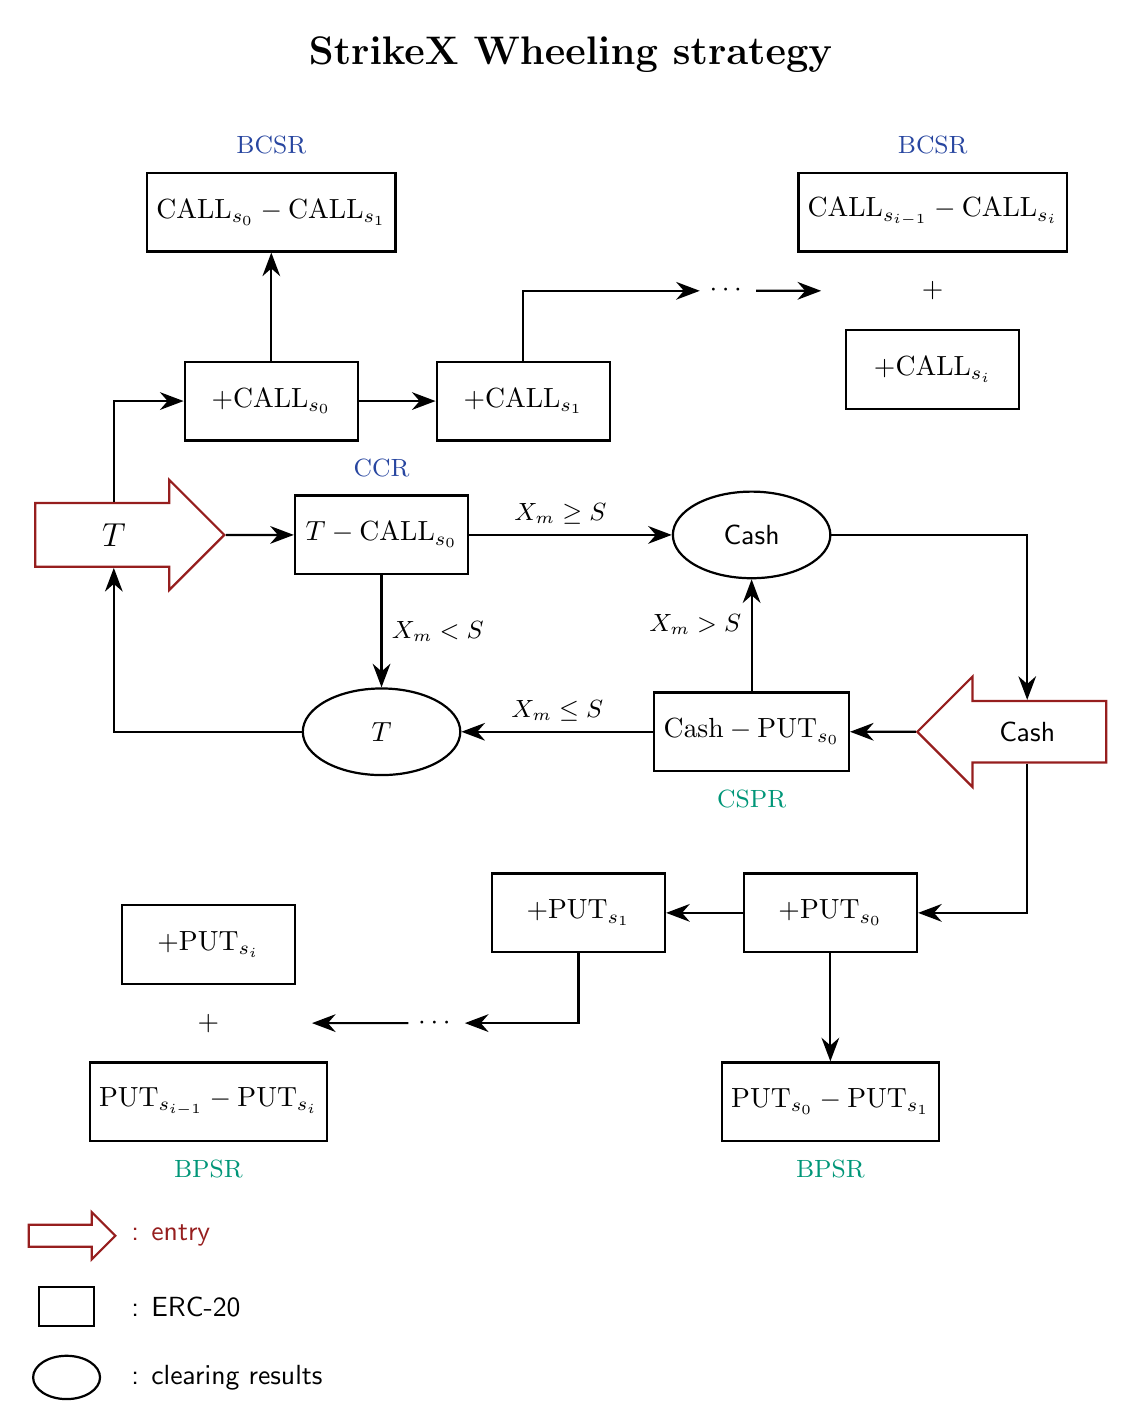
\begin{tikzpicture}[
  font=\sffamily,
  box/.style={draw, rectangle, minimum width=2.2cm, minimum height=1cm, align=center, line width=0.8pt},
  ell/.style={draw, ellipse, minimum width=2cm, minimum height=1.1cm, align=center, line width=0.8pt},
  >={Stealth[length=3mm]},
  arrline/.style={->, line width=0.8pt},
]

% ============ Graph title ============
\node[font=\Large\bfseries] at (6.4,11.0) {StrikeX Wheeling strategy};

% (T base-split equation: moved below the figure)

% ============ BCSR boxes (top) ============
\node[box] (bcsr1) at (2.6,9.0) {$\mathrm{CALL}_{s_0}-\mathrm{CALL}_{s_1}$};
\node[align=center, font=\small, color=wbblue] at (2.6,9.85) {BCSR};

\node[box] (bcsr2top) at (11.0,9.0) {$\mathrm{CALL}_{s_{i-1}}-\mathrm{CALL}_{s_i}$};
\node[align=center, font=\small, color=wbblue] at (11.0,9.85) {BCSR};
\node[box] (bcsr2bot) at (11.0,7.0) {$+\mathrm{CALL}_{s_i}$};
\node at (11.0,8.0) {$+$};

% (CALL-NP / CALL-NN payoffs: moved below the figure)

% ============ +CALL boxes (middle-upper) ============
\node[box] (callS0) at (2.6,6.6) {$+\mathrm{CALL}_{s_0}$};
\node[box] (callS1) at (5.8,6.6) {$+\mathrm{CALL}_{s_1}$};

% ============ Entry arrow T (big arrow, left) ============
\node[single arrow, draw, line width=0.8pt, minimum width=1.4cm, minimum height=2.4cm,
      single arrow head extend=2mm, color=wbred, rotate=0] (Tentry) at (0.6,4.9) {\color{black}\large $T$};

% ============ CCR: T - CALL_s0 ============
\node[box] (ccr) at (4.0,4.9) {$T-\mathrm{CALL}_{s_0}$};
\node[align=center, font=\small, color=wbblue] at (4.0,5.75) {CCR};

% ============ Cash ellipse ============
\node[ell] (cash1) at (8.7,4.9) {Cash};

% ============ T ellipse (lower) ============
\node[ell] (Tell) at (4.0,2.4) {$T$};

% ============ CSPR: Cash - PUT_s0 ============
\node[box] (cspr) at (8.7,2.4) {$\mathrm{Cash}-\mathrm{PUT}_{s_0}$};
\node[align=center, font=\small, color=wbgreen] at (8.7,1.55) {CSPR};

% ============ Cash entry arrow (right) ============
\node[single arrow, draw, line width=0.8pt, minimum width=1.4cm, minimum height=2.4cm,
      single arrow head extend=2mm, color=wbred, shape border rotate=180] (cashentry) at (12.2,2.4) {\color{black} Cash};

% ============ +PUT boxes ============
\node[box] (putS0) at (9.7,0.1) {$+\mathrm{PUT}_{s_0}$};
\node[box] (putS1) at (6.5,0.1) {$+\mathrm{PUT}_{s_1}$};
\node[box] (bpsr1) at (9.7,-2.3) {$\mathrm{PUT}_{s_0}-\mathrm{PUT}_{s_1}$};
\node[align=center, font=\small, color=wbgreen] at (9.7,-3.15) {BPSR};

% ============ General-step vertical stack (+PUT_si over PUT_{si-1}-PUT_si) ============
\node[box] (putSi) at (1.8,-0.3) {$+\mathrm{PUT}_{s_i}$};
\node at (1.8,-1.3) {$+$};
\node[box] (bpsr2) at (1.8,-2.3) {$\mathrm{PUT}_{s_{i-1}}-\mathrm{PUT}_{s_i}$};
\node[align=center, font=\small, color=wbgreen] at (1.8,-3.15) {BPSR};

% (Cash base-split equation: moved below the figure)

% (PUT-NP / PUT-NN payoffs: moved below the figure)

% ===================== ARROWS =====================

% +CALL_{s_0} fans out: spread residual (CALL_{s_0}-CALL_{s_1}) and carry (+CALL_{s_1})
\draw[arrline] (callS0) -- (callS1);
\draw[arrline] (callS0.north) -- (bcsr1.south);
% +CALL_{s_1} -> up then right (90 deg) -> ... -> middle of the general-step stack
\node (ccdots) at (8.4,8.0) {$\cdots$};
\draw[arrline] (callS1.north) |- (ccdots.west);
\draw[arrline] (ccdots.east) -- ($(bcsr2top.west)!0.5!(bcsr2bot.west)$);

% Entry T arrow up to +CALL_s0   (label C.N)
\draw[arrline] (Tentry.north) |- node[pos=0.25, left, font=\small] {} (callS0.west);
% (C.N entry weight: moved below the figure)

% Entry T -> CCR box (label C.P) -- the lower split going right into T-CALL
\draw[arrline] (Tentry.east) -- (ccr.west);

% CCR -> Cash  (Xm >= S)
\draw[arrline] (ccr.east) -- node[pos=0.45, above, font=\small] {$X_m\ge S$} (cash1.west);

% CCR -> T ellipse (Xm < S)  downward
\draw[arrline] (ccr.south) -- node[pos=0.5, right, font=\small] {$X_m<S$} (Tell.north);

% Cash -> CSPR (right loop down):  Cash to cashentry then into CSPR
\draw[arrline] (cash1.east) -| (cashentry.north);

% cashentry -> CSPR  (P.P label)
\draw[arrline] (cashentry.west) -- (cspr.east);

% CSPR -> T ellipse  (Xm <= S)
\draw[arrline] (cspr.west) -- node[pos=0.5, above, font=\small] {$X_m\le S$} (Tell.east);

% CSPR -> Cash (Xm > S) upward green
\draw[arrline] (cspr.north) -- node[pos=0.6, left, font=\small] {$X_m>S$} (cash1.south);

% cashentry -> +PUT_s0 (P.N label)
\draw[arrline] (cashentry.south) |- node[pos=0.25, right, font=\small] {} (putS0.east);
% (P.N entry weight: moved below the figure)

% putS0 -> left -> putS1
\draw[arrline] (putS0.west) -- (putS1.east);
% putS0 -> straight down -> middle of bpsr1
\draw[arrline] (putS0.south) -- (bpsr1.north);
% +PUT_{s_1} -> down then left (90 deg) -> ... -> middle of the general-step stack
\node (pcdots) at (4.7,-1.3) {$\cdots$};
\draw[arrline] (putS1.south) |- (pcdots.east);
\draw[arrline] (pcdots.west) -- ($(putSi.east)!0.5!(bpsr2.east)$);

% Tell -> back to entry T (blue feedback loop, lower)
\draw[arrline] (Tell.west) -| (Tentry.south);

% (removed return path: keep a single arrow T -> +CALL_{s_0})

% ===================== LEGEND (bottom-left) =====================
\begin{scope}[shift={(0,-4.0)}]
  \node[single arrow, draw, color=wbred, line width=0.8pt, minimum width=0.6cm,
        minimum height=1.1cm, single arrow head extend=1.5mm] (le) at (0,0) {};
  \node[anchor=west, color=wbred] at (0.7,0) {: entry};
  \node[draw, rectangle, line width=0.8pt, minimum width=0.7cm, minimum height=0.5cm] at (0,-0.9) {};
  \node[anchor=west] at (0.7,-0.9) {: ERC-20};
  \node[draw, ellipse, line width=0.8pt, minimum width=0.85cm, minimum height=0.55cm] at (0,-1.8) {};
  \node[anchor=west] at (0.7,-1.8) {: clearing results};
\end{scope}

\end{tikzpicture}%
}
\caption{Tokenized option ladder as a recursion / state machine over the underlying
state $T$ and the cash state. Red arrows are entry points; each state splits into an
obligation residual ($P$) and a right ($N$). The covered-call residual ($\CCR$) and its
mirror the cash-secured-put residual ($\CSPR$) move probability mass between the $T$ and
Cash states at maturity according to $X_m$ vs.\ the strike $S$, while the right legs
recurse along the strike ladder into bull/bear spread residuals ($\BCSR$, $\BPSR$).
This figure is the visual counterpart of the algebraic identities in Sections~3--4.}
\label{fig:ladder}
\end{figure}

\subsection*{Equations referenced in the diagram}

\textit{Base splits (one maturity step):}
\[
T = \underbrace{(T-\Call)}_{\CP} + \underbrace{\Call}_{\CN},
\qquad
\mathrm{Cash} = \underbrace{(\mathrm{Cash}-\Put)}_{\PP} + \underbrace{\Put}_{\PN}.
\]

\textit{Entry-split weights} (token / cash units; here $S$ denotes the base strike $S_0$ and $X_m$ the terminal price):
\begin{align*}
\CP &= \min\!\left(1,\tfrac{S}{X_m}\right)T, & \CN &= \max\!\left(0,1-\tfrac{S}{X_m}\right)T,\\
\PP &= \min\!\left(1,\tfrac{X_m}{S}\right)C, & \PN &= \max\!\left(0,1-\tfrac{X_m}{S}\right)C.
\end{align*}

\textit{Per-bucket spread and tail payoffs:}
\begin{align*}
\CNPi{i} &= \min\!\big(\max(0,X_m-S_{i-1}),\,S_i-S_{i-1}\big), & \CNNi{i} &= \max(0,X_m-S_i),\\
\PNPi{i} &= \min\!\big(\max(0,S_{i-1}-X_m),\,S_{i-1}-S_i\big), & \PNNi{i} &= \max(0,S_i-X_m).
\end{align*}

% =====================================================================
\section{Summary}
% =====================================================================

\subsection*{Compact identities}

\textit{Call side, increasing strikes $S_0<S_1<\cdots<S_n$ (conserves to $X_m$):}
\begin{align}
X_m
&= \underbrace{\min(X_m,S_0)}_{\text{covered-call residual}}
+ \sum_{i=1}^{n}\underbrace{\min\!\left(\max(0,X_m-S_{i-1}),S_i-S_{i-1}\right)}_{\text{bull call spread residual}}
+ \underbrace{\max(0,X_m-S_n)}_{\text{tail call}}.
\end{align}

\textit{Put side, decreasing strikes $S_0>S_1>\cdots>S_n$ (conserves to $S_0$):}
\begin{align}
S_0
&= \underbrace{\min(X_m,S_0)}_{\text{cash-secured-put residual}}
+ \sum_{i=1}^{n}\underbrace{\min\!\left(\max(0,S_{i-1}-X_m),S_{i-1}-S_i\right)}_{\text{bear put spread residual}}
+ \underbrace{\max(0,S_n-X_m)}_{\text{tail put}}.
\end{align}

\subsection*{Master tranche reference}

\begin{longtable}{>{\raggedright\arraybackslash}p{0.25\linewidth}p{0.65\linewidth}}
\toprule
Label & Formula / meaning \\
\midrule
$\CP$ / $\CCR$ & Covered call residual: $\min(X_m,S_0)$. \\
$\CN$ & Call right (long call): $\max(0,X_m-S_0)$. \\
$\CNP$ / $\BCSR$ & Bull call spread residual: $\min(\max(0,X_m-S_{i-1}),S_i-S_{i-1})$. \\
$\CNN$ & Higher-strike tail call: $\max(0,X_m-S_i)$. \\
$\PP$ / $\CSPR$ & Cash-secured put residual: $\min(X_m,S_0)$. \\
$\PN$ & Put right (long put): $\max(0,S_0-X_m)$. \\
$\PNP$ / $\BPSR$ & Bear put spread residual: $\min(\max(0,S_{i-1}-X_m),S_{i-1}-S_i)$. \\
$\PNN$ & Lower-strike tail put: $\max(0,S_i-X_m)$. \\
\bottomrule
\end{longtable}

\todo{Master worked example combining both sides + the wheel cycle across two maturities (extends the per-side numerical checks of Sections~3.4 and~4.4).}

\end{document}
